\subsection{Saboteur - Lựa chọn trong vô vàn board game}

Board game Saboteur ra mắt năm 2004, được thiết kế bởi Fréderic Moyersoen, nhanh chóng trở thành một trong những trò chơi nhóm nổi tiếng nhất nhờ lối chơi bluffing - tương tác - phản bội cực kỳ kịch tính. Lấy bối cảnh những người thợ mỏ cùng nhau đào đường hầm tìm kho báu nhưng luôn có kẻ phá hoại ẩn mình, Saboteur tạo nên sự pha trộn hoàn hảo giữa chiến thuật, đọc vị tâm lý và những màn phản đòn bất ngờ. Nhờ luật chơi đơn giản nhưng độ sâu chiến thuật cao, trò chơi phù hợp với nhiều độ tuổi và được dịch, phát hành rộng rãi trên toàn thế giới. Với tính chất tương tác mạnh và khả năng tạo ra vô số tình huống hài hước lẫn “plot twist”, Saboteur hoàn toàn xứng đáng được tái hiện trong một trò chơi online 3D nhiều người chơi, nơi người chơi không chỉ chơi bài mà còn giao tiếp, hành động và trải nghiệm cảm giác nghi kỵ - hợp tác sống động hơn bao giờ hết trong không gian cabin ảo.

\begin{figure}[H]
    \centering
    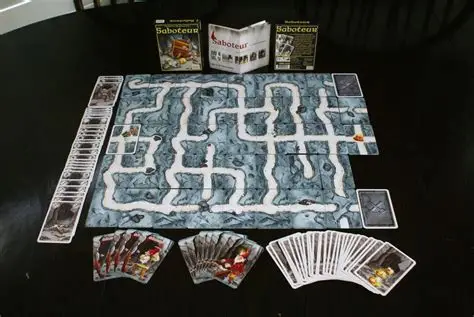
\includegraphics[width=0.75\linewidth]{5.Thiết kế//images/image.png}
    \caption{Bộ bài Saboteur đầy đủ}
    \label{fig:placeholder}
\end{figure}

Luật chơi của Saboteur \cite{saboteur2024} cụ thể như sau:

\begin{enumerate}
\item \textbf{Tổng quan và mục tiêu}

\begin{itemize}
  \item Số người chơi: 3--10.
  \item Mục tiêu:
  \begin{itemize}
      \item \textbf{Gold-Diggers}: mở đường từ Start đến Goal chứa vàng.
      \item \textbf{Saboteurs}: phá để Gold-Diggers không thể đến được vàng.
  \end{itemize}
\end{itemize}

\item \textbf{Trang bị trong bộ Saboteur}

\begin{itemize}
  \item 40 Thẻ đường (path cards): gồm 31 thẻ thông, 9 thẻ cụt
  \item 27 Thẻ hành động (action cards)
  \item 11 Thẻ vai trò (role cards)
\end{itemize}


\item \textbf{Bố trí bàn chơi (Setup)}

\begin{figure}[H]
    \centering
    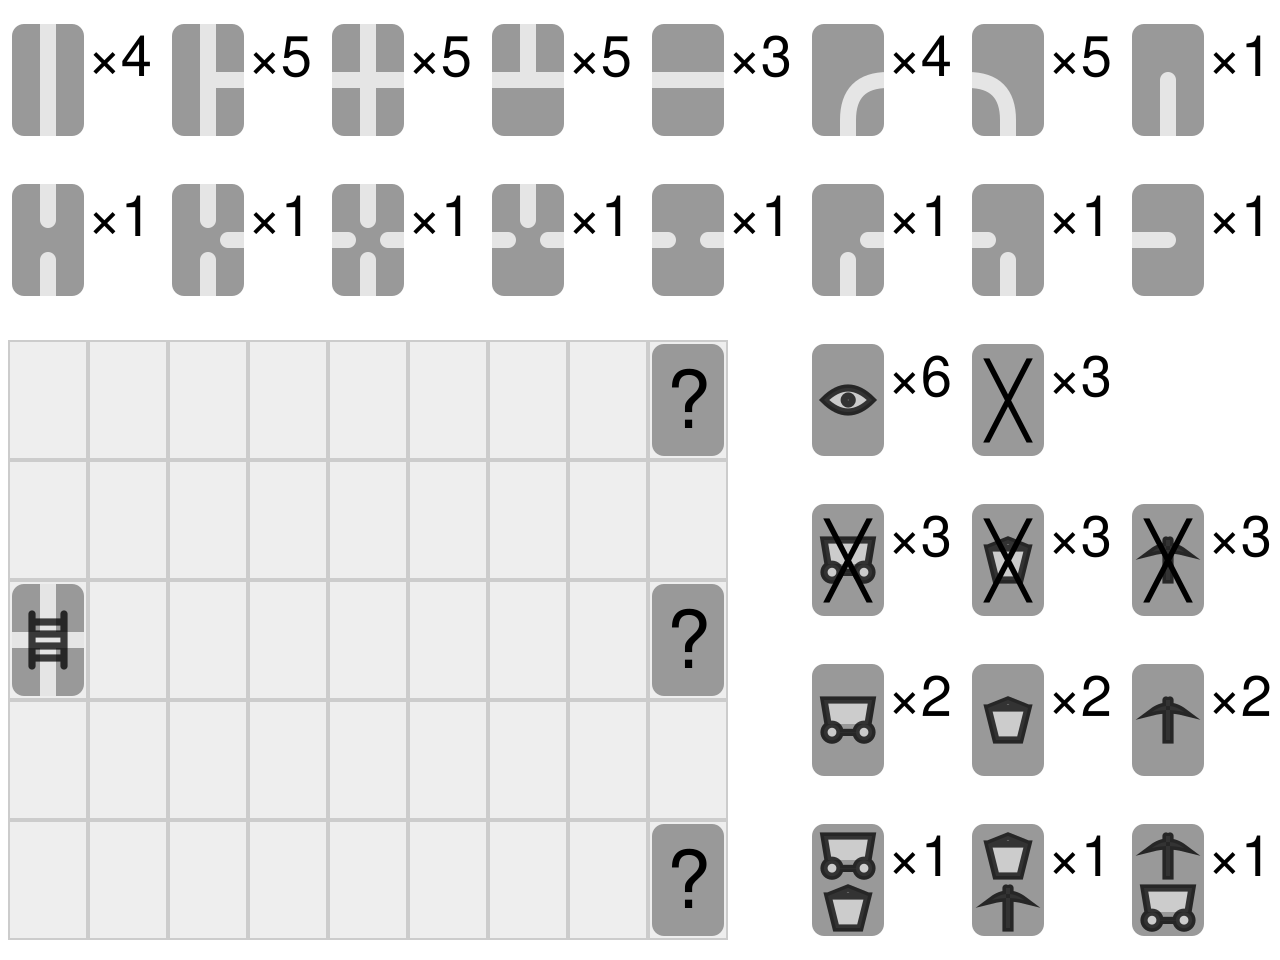
\includegraphics[width=0.75\linewidth]{5.Thiết kế//images/saboteurCards.png}
    \caption{Hình minh họa bộ thẻ và bàn chơi}
    \label{fig:cards-and-board}
\end{figure}


\begin{itemize}
  \item Đặt thẻ Start ở giữa bên trái.
  \item Đặt 3 thẻ Goal úp cách Start 7 khoảng thẻ: 1 giữa, 1 trên, 1 dưới.
  \item Vai trò và số thẻ phát cho mỗi người\\
  % \textbf{Số lượng vai trò theo số người chơi:}
    \begin{table}[h]
    \centering
        \begin{tabular}{|c|c|c|c|c|c|c|c|c|}
        \hline
        Tổng số Người chơi & 3 & 4 & 5 & 6 & 7 & 8 & 9 & 10 \\ \hline
        Số Saboteurs     & 1 & 1 & 2 & 2 & 3 & 3 & 3 & 4 \\ \hline
        Số Gold-Diggers  & 2 & 3 & 3 & 4 & 3 & 4 & 5 & 6 \\ \hline
        \end{tabular}
        \caption{Bảng số lượng vai trò theo số người chơi:}
        \label{tab:total-roles}
    \end{table}
    % \textbf{Số thẻ phát cho mỗi người:}
    \begin{table}[h]
    \centering
        \begin{tabular}{|c|c|c|c|c|c|c|c|c|}
        \hline
        Tổng số Người chơi      & 3 & 4 & 5 & 6 & 7 & 8 & 9 & 10 \\ \hline
        Thẻ mỗi người      & 6 & 6 & 6 & 5 & 5 & 4 & 4 & 4 \\ \hline
        \end{tabular}
        \caption{Bảng số thẻ phát cho mỗi người}
        \label{tab:cards-per-player}
    \end{table}

    \item Tất cả những lá bài còn lại được xáo lại thành chồng và để úp xuống bàn.
\end{itemize}


\item \textbf{Luật chơi}

\begin{itemize}
  \item Lượt xoay chiều kim đồng hồ.
  \item Mỗi lượt chọn một trong các hành động:
  \begin{enumerate}
    \item Đặt thẻ đường (path card).
    \item Chơi thẻ hành động (action card).
    \item Bỏ thẻ (discard).
  \end{enumerate}
  \item Sau khi xong lượt của mình, người chơi bốc lên thẻ trên cùng của deck, lượt chơi tiếp tục qua người tiếp theo.
  \item Gold-Diggers thắng khi có đường nối (phải là đường thông) từ start tới goal chứa vàng. Saboteurs thắng khi tất cả đã hết bài mà vẫn chưa nối được đường tới vàng.
\end{itemize}

% ========================================================
% 6. PATH CARDS
% ========================================================
\item \textbf{Thẻ đường (Path Cards)}
\begin{figure}[H]
    \centering
    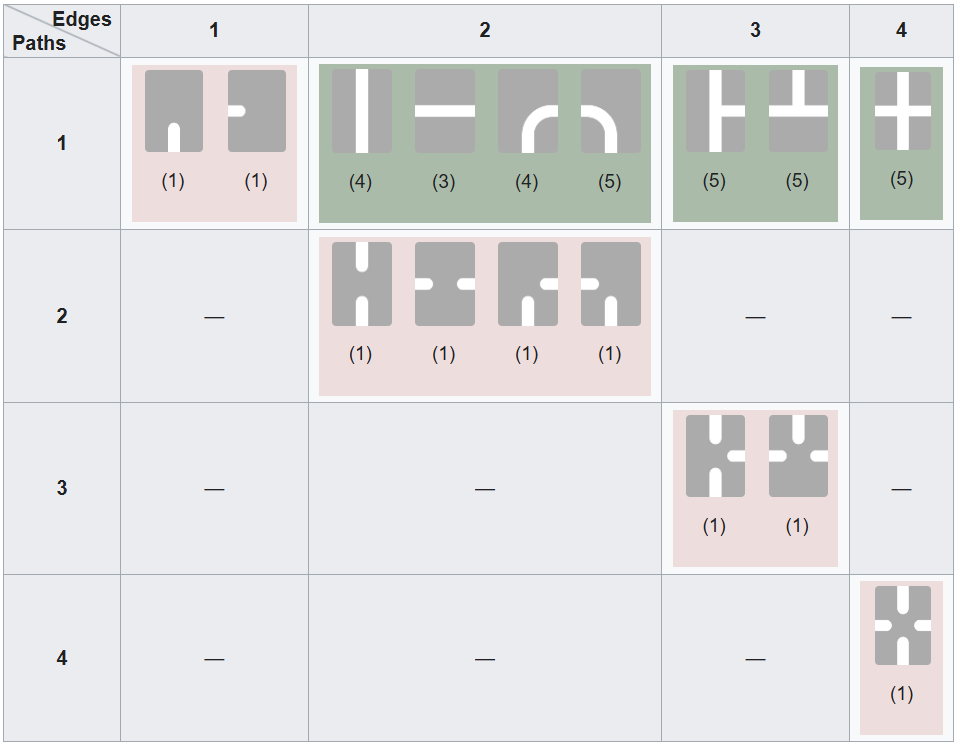
\includegraphics[width=0.75\linewidth]{5.Thiết kế//images/pathCards.png}
    \caption{Phân loại thẻ đường}
    \label{fig:placeholder}
\end{figure}
% \fbox{\parbox[c][4cm][c]{0.85\textwidth}{\centering (Placeholder) Các loại path cards}}
\begin{itemize}
  \item \textbf{Phân loại thẻ Đường}  
  Thẻ Đường (\emph{Path cards}) trong Saboteur được dùng để tạo ra mạng lưới đường hầm từ vị trí xuất phát đến các thẻ mục tiêu. Chúng được chia thành:
  \begin{itemize}
    \item \textbf{Thẻ đường thẳng}: nối liền hai đầu theo trục ngang hoặc dọc.
    \item \textbf{Thẻ giao nhau}: có nhiều nhánh rẽ, cho phép mở rộng đường theo nhiều hướng.
    \item \textbf{Thẻ cụt (dead-end)}: Có thể nối với các thể khác nhưng không được tính là thông đường.
    \item \textbf Các cạnh thẻ không có lối được tính là tường,  khiến người chơi không thể nối đường theo hướng đó.
  \end{itemize}

  \item \textbf{Cách đặt thẻ Đường hợp lệ}  
  Một thẻ Đường được xem là hợp lệ khi thỏa các điều kiện sau:
  \begin{itemize}
    \item Các đầu đường (lối ra) trên thẻ mới phải khớp với đầu đường của thẻ đã có trên bàn: đường nối với đường, tường nối với tường.
    \item Không được tạo ra một kết nối trái ngược (ví dụ: đầu đường mở nối vào tường bịt).
    \item Thẻ phải được đặt kề cạnh một thẻ đã có sẵn trong mạng lưới (không được “nhảy cóc”).
    % \item Người chơi không được phá vòng lặp đang tồn tại trừ khi dùng thẻ hành động chuyên biệt.
  \end{itemize}

  \item \textbf{Quy tắc xoay thẻ}  
  Tất cả thẻ Đường đều có thể được xoay 180° trước khi đặt xuống.  
  \begin{itemize}
    \item Người chơi không được xoay 90°; chỉ xoay 180° vì cấu trúc hầm được thiết kế theo hai hướng chính.
    \item Sau khi xoay, thẻ vẫn phải thỏa điều kiện kết nối hợp lệ như đã nêu ở mục trên.
  \end{itemize}

  \item \textbf{Phá đường bằng thẻ Bomb}  
  Thẻ \emph{Bomb} là thẻ hành động dùng để phá hủy một thẻ Đường đã được đặt trên bàn.
  \begin{itemize}
    \item Người chơi chọn một thẻ Đường bất kỳ (trừ thẻ Start và thẻ Goal) để loại bỏ.
    \item Sau khi phá, ô trống được để lại và không có thẻ nào tự động dịch chuyển vào.
    \item Bomb không được dùng để phá thẻ trên tay người chơi, chỉ phá thẻ đã đặt.
  \end{itemize}

\end{itemize}
% ========================================================
% 7. ACTION CARDS
% ========================================================
\item \textbf{Thẻ hành động (Action Cards)} 

Các thẻ hành động ảnh hưởng trực tiếp đến khả năng đặt thẻ đường hoặc quan sát thông tin trong ván chơi.  
Trong game có \textbf{3 loại công cụ}: 
\begin{itemize}
    \item Xe đẩy (\textit{Cart})
    \item Xẻng (\textit{Shovel})
    \item Mũ (\textit{Hat})
\end{itemize}

Nếu người chơi bị phá \textbf{bất kỳ một trong ba công cụ}, họ \textbf{không thể đặt thẻ đường}.  
Để sửa, người chơi phải dùng thẻ Repair tương ứng.

\begin{itemize}
    \item \textbf{Repair đơn}: sửa đúng 1 công cụ được chỉ định trên thẻ.
    \item \textbf{Repair kép}: sửa 1 trong 2 công cụ hiển thị trên thẻ (Có biến thể có thể sửa cả hai đồng thời).
\end{itemize}

\begin{table}[H]
\centering
\begin{tabular}{|c|p{7cm}|c|}
\hline
\textbf{Loại thẻ} & \textbf{Công dụng} & \textbf{Số lượng} \\ \hline
Sabotage & Phá 1 công cụ: Cart, Shovel hoặc Hat. Người bị phá không thể đặt Path cho đến khi được sửa. & 9 \\ \hline
Repair   & Sửa công cụ bị phá. Gồm: 6 thẻ đơn (mỗi loại công cụ 2 thẻ), 3 thẻ kép. & 9 \\ \hline
Map      & Cho phép xem lén 1 trong 3 thẻ Goal. Không được tiết lộ thông tin trừ khi tự nguyện. & 6 \\ \hline
Rockfall & Phá hủy 1 Path card trên bàn (trừ Start và 3 Goal). Thẻ bị phá được loại khỏi mỏ. & 3 \\ \hline
\end{tabular}
\end{table}

% \end{itemize}

\end{enumerate}